\section{Method: Action Design Research - Drools in MPS}
\label{section:Method_action_research}

Even though Drools is a relatively small DSL, we did not need to implement all the functionality to answer our questions.

\subsection{Really Simple Rules Language}
As we were new to DSL design and MPS, we first would create a simple approximation of the Drools language to create our first projections.
We called this language ``Really Simple Rules'' (RSR).

\paragraph{File} RSR, Like Drools itself, has a File as its root node.
The File only contains Facts and Rules.

\paragraph{Fact and FactProperty} In Drools, a fact represents a Java Bean with its child properties, which can also have their child properties, ad infinitum.
In RSR, we limited properties to allow only boolean values.
We decided this because fact selection is a predicate and thus can only return a boolean.
By only allowing booleans, we also simplify the operations allowed on the property.

\paragraph{Rule} We only simulated the Left Hand Side, or the ``When'' conditions, of a Drools Rule for the Rules Concept.
We believed this would provide us with compelling options for projections and did not want to overcomplicate this first approach.

An RSR Rule consists of a collection of conditions.
Should all those conditions return true, then the rule is selected.

\paragraph{Condition} A condition operates on one or more FactSelectors.
There are four condition types ExistsCondition, NotCondition, AndCondition, and OrCondition.
ExistsCondition and NotCondition are unary conditions and evaluate one FactSelector.
AndCondition and OrCondition conditions evaluate two FactSelectors.

\paragraph{FactSelector} A FactSelector consists of a reference to a Fact and a collection of Predicates.
If the Fact exists and all the predicates evaluate to true, then the FactSelector evaluates to true.

\paragraph{Predicate} The predicate is an operation on a FactProperty, to which the Concept has a reference.
Because FactProperty represents a boolean value, the only predicate operations are ``Is'' and ``Not''.

Figure \ref{fig:RSRDiagram} shows the Concept hierarch for this straightforward implementation.

\begin{figure}[h]
    \centering
    \fbox{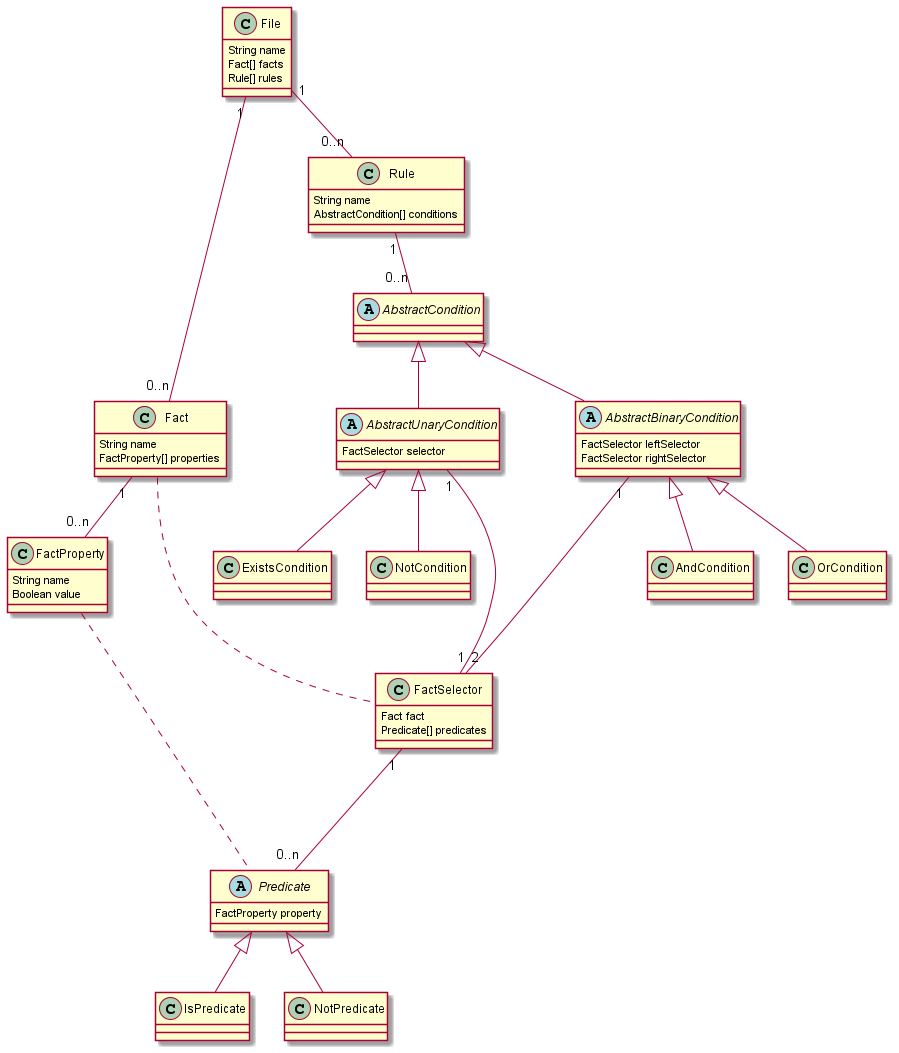
\includegraphics[width=0.95\textwidth]{Sections/images/ReallySimpleRuleLanguage.png}}
    \caption{RSR concept hierarchy}
    \label{fig:RSRDiagram}
\end{figure}

We realised this design in MPS.
As the aim is to attempt different projections, we did not initially optimise for editing.
The structure is as shown in figure \ref{fig:RSRStructure}, and the editors, including those shown in figure \ref{fig:RSREditors}.

\begin{figure}
    \centering
    \begin{minipage}{0.30\textwidth}
        \centering
        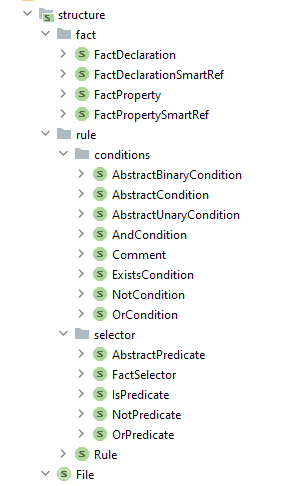
\includegraphics[width=0.9\textwidth]{Sections/images/RSRStructrure.png}
        \caption{RSR}
        \label{fig:RSRStructure}
    \end{minipage}\hfill
    \begin{minipage}{0.70\textwidth}
        \centering
        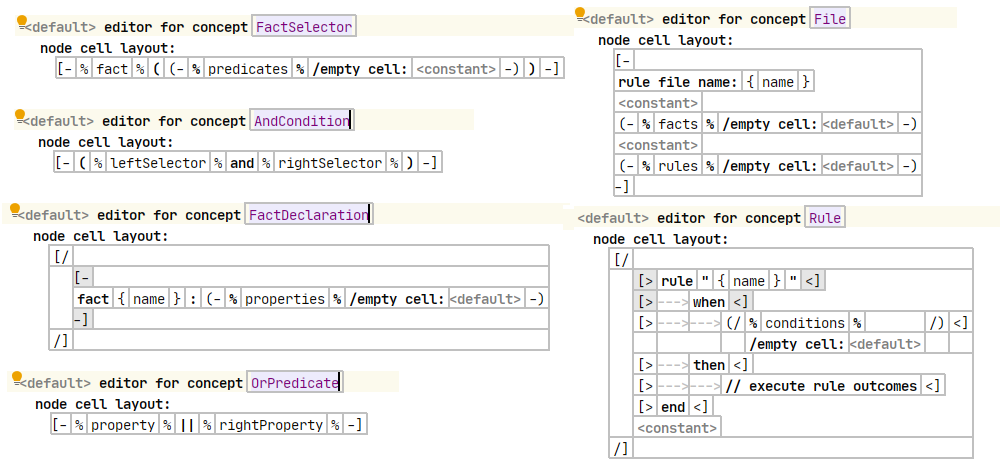
\includegraphics[width=0.9\textwidth]{Sections/images/RSREditors.png} 
        \caption{Editors}
        \label{fig:RSREditors}
    \end{minipage}
\end{figure}

Part of the research question is using projections for reasoning about large files.
In order to answer this, we needed to simulate a large file.
To do this, we had to enter a large number of rules.
As this becomes tedious, we added some editing aids, including substitute menus, to speed up the entry of conditions, as shown in figure \ref{fig:RSRSubstituteMenu}.

This image shows that we originally had to select an ExistsCondition Concept and select the Fact for the condition.
After adding the substitute menu, We could immediately select the Fact we wanted, and the ExistsCondition would automatically wrap it with an ExistsCondition node.

\begin{figure}[h]
    \centering
    \fbox{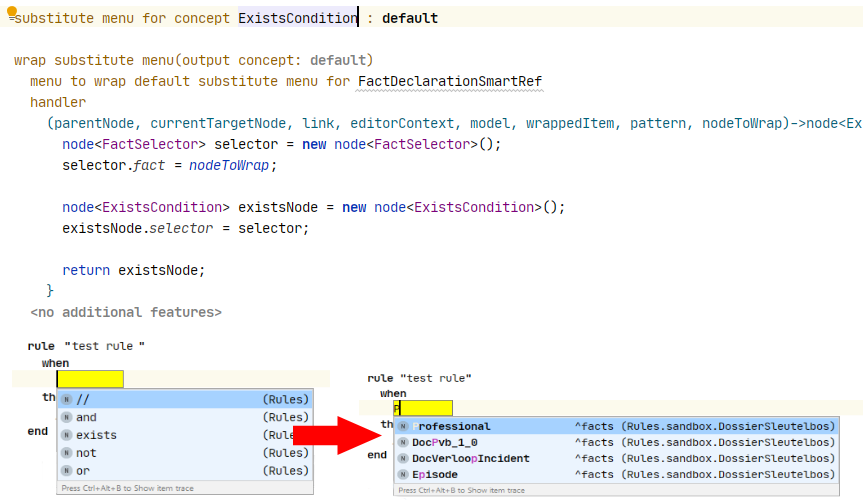
\includegraphics[width=0.95\textwidth]{Sections/images/RSRSubstituteMenu.png}} 
    \caption{RSR substitute menu}
    \label{fig:RSRSubstituteMenu}
\end{figure}

We also added some intentions to invert incorrectly added conditions.

Finally, we added a Constraint to scope the fact properties in predicates to the Fact chosen in the FactSelector.
This scope Constraint made it much easier to select properties in the predicates as indicated in figure \ref{fig:RSRConstraint}.

The figure shows that before adding the scoping constraint, it showed a list with dozens of potential FactProperties, that represented all the FactProperties in the Model.
After adding the constraint, it only shows the two properties associates with the Fact from the FactSelector.

\begin{figure}[h]
    \centering
    \fbox{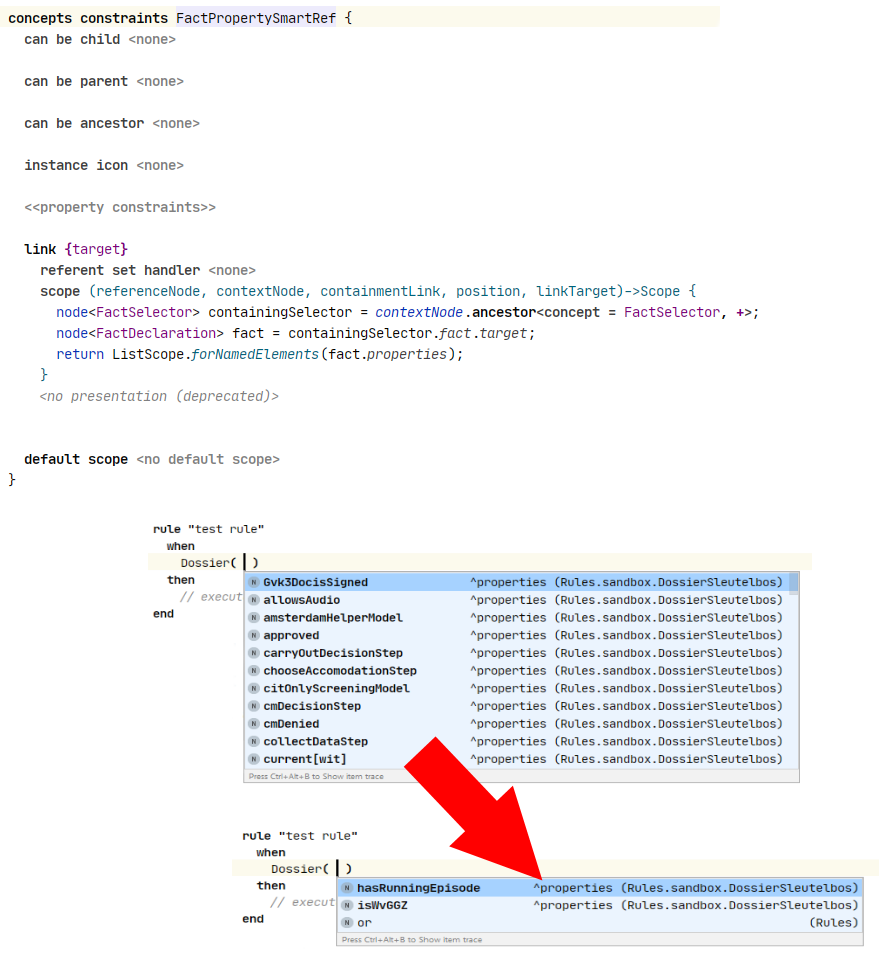
\includegraphics[width=0.95\textwidth]{Sections/images/RSRConstraint.png}}
    \caption{RSR scoping constraint}
    \label{fig:RSRConstraint}
\end{figure}

Thus, we have described the entire implementation of the Really Simple Rules Language.

After implementing the language, we wrote a program with a large number of rules.
This program on which we will experiment with the different projections.
Figure \ref{fig:RSRProgram} shows an example of our default Drools like text projection.

\begin{figure}[h]
    \centering
    \fbox{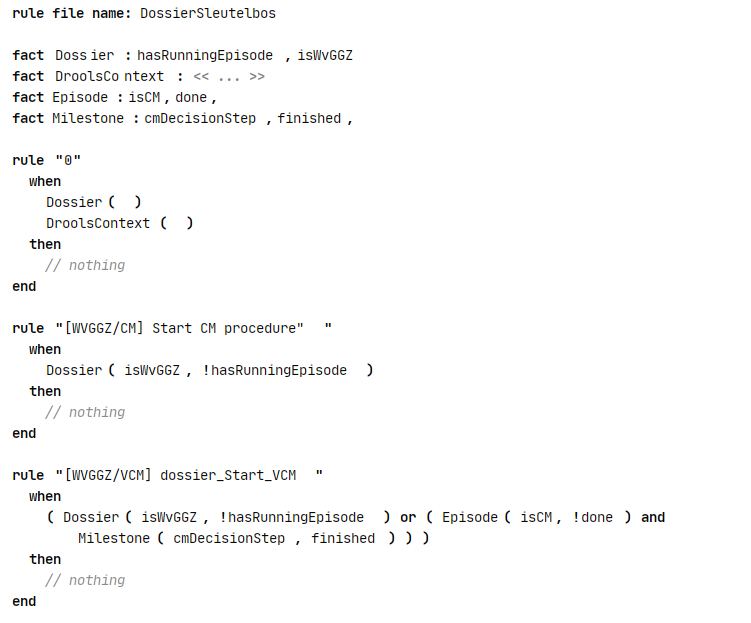
\includegraphics[width=0.95\textwidth]{Sections/images/RSRProgram.png}}
    \caption{RSR program}
    \label{fig:RSRProgram}
\end{figure}

We discuss the alternative projections in the results section \ref{section:Results_ADR}.

\subsection{Drools-Lite Language}
\label{section:DroolsLite}

The RSR was useful as an initial language. 
However, it suffered from two significant issues.
Firstly, its limitations as a language were so substantial that it could not handle many necessary scenarios.
Secondly, our projections would have to be validated by developers with Drools experience.
For this reason, we needed to create a projectional language that was much closer to the Drools language.

Our following Language, Drools-Lite, contains many more of the features of Drools.
Our method of selecting the features involved implementing the examples delivered with Drools (including the corrupt politician example shown in section \ref{section:WhatIsDrools}).
We would implement just enough features to complete the examples.
Whenever we had any queries about how to design the Concepts, we referred to our analysis of the Drools Language, shown in appendix \ref{appendix:DroolsConceptHierarchy}.
We show the preliminary design we achieved using this method in figure \ref{fig:DroolsLiteDiagram}.
Later, there were some places we diverged a little from our design.
We merged and decoupled our Concepts when we thought it would simplify the code.

\begin{figure}[htbp]
    \centering
    \fbox{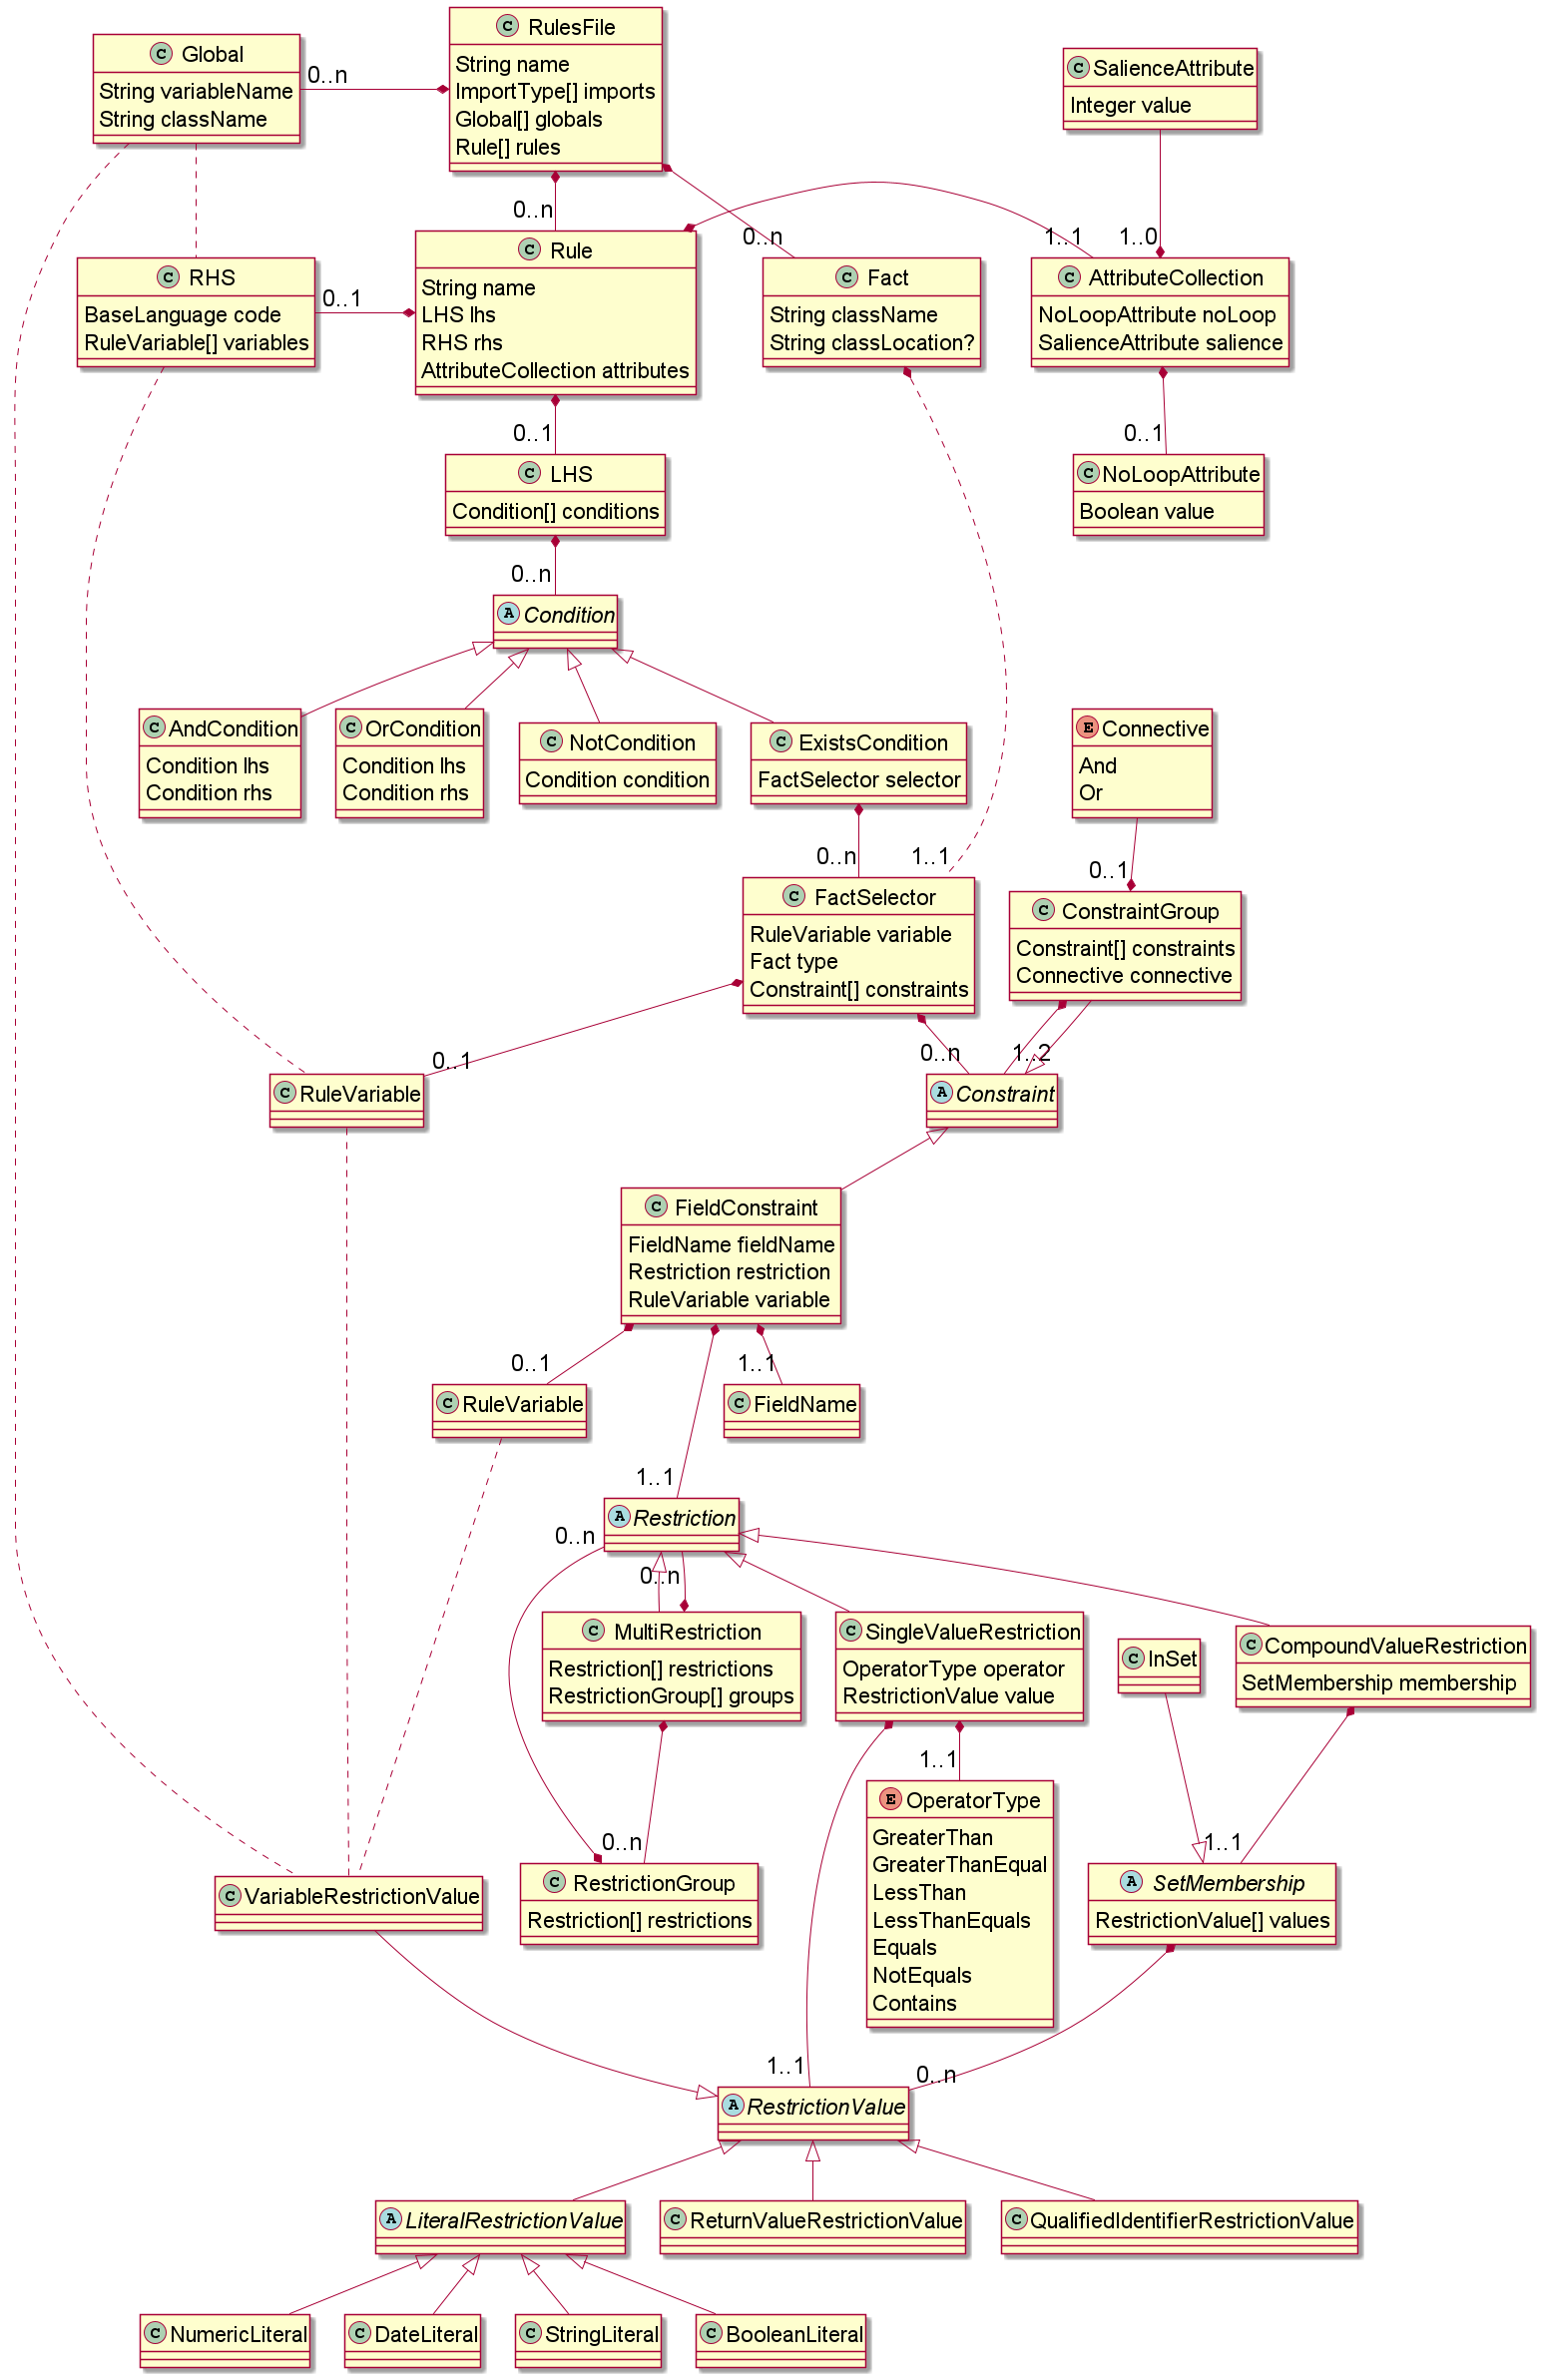
\includegraphics[width=0.85\textwidth]{Sections/images/DroolsLiteStructure.png}}
    \caption{Drools-Lite structure}
    \label{fig:DroolsLiteDiagram}
\end{figure}
 
\paragraph{RuleFile} The RuleFile level statements contain Facts, Globals and Rules.
It also contains semantically unimportant empty lines.

\paragraph{Fact} A Fact has a type property.
We implement the type property using a ClassifierType from the MPS BaseLanguage.
This implementation allows the File to refer to BaseLanguage classes implemented in the same solution and Java JAR files.
We created a smart reference Concept for this to take advantage of built-in MPS UI functionality.
A smart reference is a node with a single reference of 1:1 cardinality.
The editor builders know how to select which nodes in scope to display to the developer if one uses this object rather than directly referencing the node to which it refers.

\paragraph{FactProperty} In RSR, we had FactProperties as children of Facts.
Now that our Facts refer to actual classes (ClassifierType), our FactProperties should reflect this.
To do this, the Concept itself only references an InstanceMethodDeclaration, the MPS BaseLanguage's definition of a Method signature.
We scoped the Concept to only show properties associated with a selected Fact.

Drools interacts with Java objects as if they are Java Beans.
To simulate this, we limited the scope of the properties to just getters, i.e. methods that start with ``get'' or ``is'' and used a Behavior to make sure they displayed without the ``get'' or ``is'' prefix.
We also made a smart reference for this Concept.

Another option for achieving this is to have wrapped the ClassifierType and referenced its related InstanceMethodDeclarations.
We would have then had to limit the functionality of these items from the BaseLanguage.
Whilst this allows the functionality we wished for, we feel our construction offers decoupling and that we think correctly reflects the structure of the language.
Perhaps if we were to redo this, we would have taken the other approach.

\paragraph{Global} Our Globals are very simple.
They have a name and a BaseLanguage Type.
We added a smart reference so that Rules can easily use them.
The reference extended Expression from the BaseLanguage.
This extension is so that we could use it in the Right-hand side.

\paragraph{Rule} Our Rules have three children: an Attribute collection, a Right Hand Side and a list of Conditions that make up the Left-hand side.
We created a component to describe the rule editor for reuse, as we imagined that we would wrap this in other projections.

\paragraph{RuleVariables} The Fact of a FactSelector and the FactProperty of a FieldConstraint are bound to RuleVariables.
RuleVariables are scoped to a Rule.
A RuleVariable has only a name and a type.
We also create a smart reference for it so that it can be used elsewhere within the rule.
Like the Global, it extends BaseLanguage's Expression to be available in the Java code of the Right-hand side.

\paragraph{Right-Hand Side} The right-hand side of the rule, for the most part, is Java code.
To implement this, we made the right-hand side of the rule a single StatementList.
A StatementList is a list of Statements, both from the BaseLanguage.
We chose these because they keep track of, amongst other things, scope.

There are some non-Java, Drools specific items that are available to the right-hand side.
Items that had to be useable within the right-hand side were Globals, RuleVariables and Drools specific functions.
These all extend Expression from the BaseLanguage.
This extension allows seamless integration with the Java code.

The Drools specific Methods that are required are Insert, InsertLogical, Modify, Delete and Halt.

\begin{figure}[!h]
    \centering
    \fbox{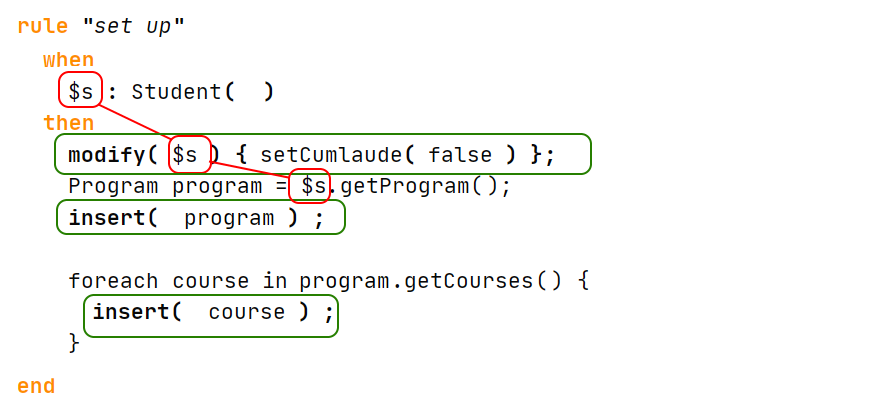
\includegraphics[width=0.70\textwidth]{Sections/images/RHS.png}}
    \caption{RHS}
    \label{fig:RHS}
\end{figure}

Figure \ref{fig:RHS} shows some of the features discussed for the right-hand side as shown in our default projection.
The right-hand side is the text shown between the \texttt{then} keyword and the \texttt{end} keyword.
In the figure, one can see examples of plain Java code, such as assigning to the variable \texttt{program} and the \texttt{foreach} loop.
We can also see that Drools-Lite RuleVariable \texttt{\$s} is in the Java statements.
We have also highlighted the Drools specific methods placed in the code, in this case \texttt{\textbf{modify}} and \texttt{\textbf{insert}}   

\paragraph{RuleAttributes} Rule Attributes is a container to hold all of the attributes that apply to a rule.
Initially, we have only implemented the No-Loop and Salience Attributes.
A developer activates these Attributes using two intentions we added to the Rule Concept.
We can see, on line 2 in figure \ref{fig:Rule}, an example of the salience attribute added to a rule on line 2.
\footnote{In figure \ref{fig:Rule}, we added line numbers to this figure to make it easier to talk about.
The keywords \texttt{rule} on line 1, \texttt{when} on line 3, \texttt{then} on line 6, and \texttt{end} on line 8 have no meaning in the abstract syntax.
We added them to give the developer the same look and feel as a standard Drools file.}

\begin{figure}[h]
    \centering
    \fbox{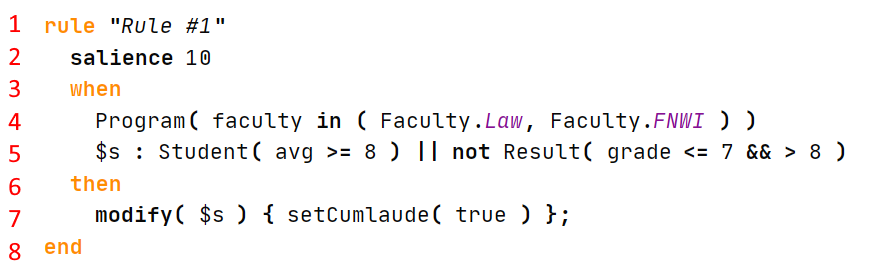
\includegraphics[width=0.85\textwidth]{Sections/images/Rule.png}}
    \caption{Rule}
    \label{fig:Rule}
\end{figure}

\paragraph{Left-Hand Side} This is a collection of conditions.
There are four types of conditions.
AndCondition, OrCondition, NotCondition and ExistsCondition.
AndCondition, OrCondition, and NotCondition have one or two children who are also conditions.
The ExistsCondition contains a FactSelector.

We added dynamic braces to only show braces around a Condition if a child of another Condition.
These braces add visual clarity without adding unnecessary clutter.
We also added some intentions to make it easy to switch between ExistsCondition and NotCondition.

On line 4 in figure \ref{fig:Rule}, the whole line represents an Exists Condition.
Line 5 shows an OrCondition containing an ExistsCondition and a NotCondition.
The default editor, through an intention, can make the ExistsCondition explicit with an \texttt{exists} keyword.
However, the standard practice with Drools developers is to make this implicit, so this is how we show it here.

\paragraph{FactSelector} This always has a reference to a fact.
These facts are \texttt{Program} in line 4 of figure \ref{fig:Rule}, and \texttt{Student} and \texttt{Result} from line 5.

Optionally, the FactSelector can be bound to a variable.
In figure \ref{fig:Rule} line 5 the FactSelector referencing the \texttt{Student} Fact is bound to the \texttt{\$s} variable.

The FactSelector also contains a list of constraints on FactProperties, that all must return true for the FactSelector to return true.

\paragraph{Constraints} We have three types of constraints.
AndConstraint and OrConstraint contain other constraints.
The FieldConstraints places restrictions on FactProperties.

\paragraph{FieldConstraints} A FieldConstraint refers to a FactProperty and can be bound to a variable.
It also has a restriction applied to that FactProperty.
Using a substitute menu, we wrapped the FactProperty smart reference.
This substitution automatically creates the FieldConstraint from the FactProperty selection by the developer.

There are several types of Restrictions and several types of values that they can restrict.

\paragraph{RestrictionValues} The RestrictionValues that a property can be compared with are as follows.
LiteralRestrictions: These are Integer, Float, String, DateTime and Boolean.
VariableRestrictions: These can be global variables, RuleVariables referring to Facts from the FactSelector, or RuleVariables from other FieldConstraints.
ReturnValue: This compares to anything expressed as an expression, which includes referring to constants or values behind qualified identifiers.

In figure \ref{fig:Rule} on line 4 we have the return values \texttt{Faculty.Law} and \texttt{Faculty.FNWI}.
on line 5 the literal values \texttt{7} and \texttt{8}.

\paragraph{Restrictions} A SingleValueRestriction compares a FactProperty against a value.
A MultiRestriction compares a FactProperty against multiple values, not necessarily using the same comparison for each value.
A SetMembership restriction checks if a FactProperty is a member of a group.

In figure \ref{fig:Rule} on line 4 a SetMembership restriction is shown with the \texttt{in ( Faculty.Law, Faculty.FNWI )} text.
Line 5 in the first FactSelector there is the SingleValue restriction \texttt{ avg >= 8}.
The second FactSelector shows a MultiRestrictions \texttt{grade <= 7 \&\& > 8}.

Thus, we have described the pertinent implementation details of the Drools-Lite language.

\subsection{Wireframes}

There are some potential projections we have conceived for which there is not sufficient time to implement.
We want others to assess these and thus would like them to appear as realistic as possible to the assessors.

Our solution to this conundrum is to develop these presentations in a wireframing tool.
The Wireframe tool we chose was Axure\cite{Axure_ProductPage}.
We chose this because we had previous experience with the product.
Also, it is available to students for free.

After much discussion, we settled on two possible projectional programming aids: Truth table and circuit diagram.
We will discuss these in more detail in the results section.
